\newpage
\section{\label{Geometry}Geometric Modeling}
\markright{\arabic{section}. Geometric Modeling}

EusLisp adopts {\emx Brep} (Boundary Representation) as the internal
representation of 3D geometric models.
Components in Breps are represented by classes
{\bf edge, plane, polygon, face, hole,} and {\bf body}.
Primitive body creating functions and body composition functions
create new instances of these classes.
In order to use your private geometric classes having
more attributes,
set special variables
{\bf *edge-class*, *face-class*} and {\bf *body-class*}
to your class objects.

\begin{figure}[htb]
\begin{center}
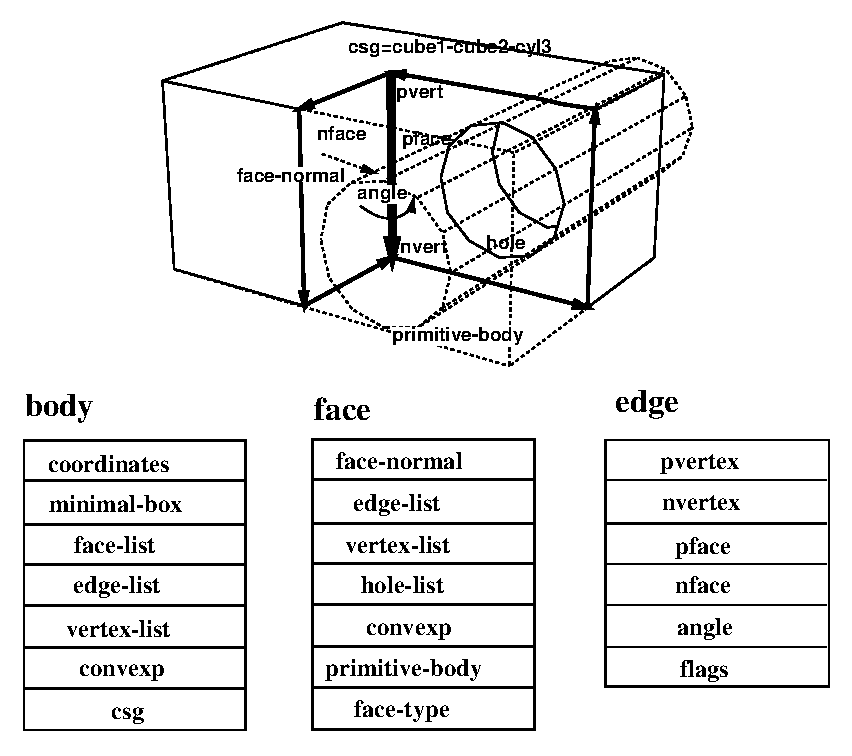
\includegraphics[height=10cm]{fig/beam.ps}
%\epsfile{file=fig/beam.ps,height=10cm}
%\mbox{
%\epsfsize=10cm
%\epsfbox{fig/beam.ps}
%% \epsfbox[0 600 300 800]{fig/beam.ps}
%}
\end{center}
\caption{Arrangements of vertices, edges, and faces}
\end{figure}

\subsection{Miscellaneous Geometric Functions}

\begin{refdesc}

\funcdesc{vplus}{vector-list}{
returns a newly created float-vector that is the sum of
all the elements of {\em vector-list}.
The difference from {\bf v+} is that {\bf vplus} computes
the sum of more than two arguments and no result vector can be specified.}

\funcdesc{vector-mean}{vector-list}{
returns the mean vector of {\it vector-list}.}

\funcdesc{triangle}{a b c \&optional (normal \#f(0 0 1))}{
{\em a, b, c} are float-vectors representing 2 or 3 dimensional points.
normal is the normal vector of the plane on which {\em a,b}, and {\em c}
lie.
{\bf Triangle} returns 2*area of a triangle formed by {\em a,b,c}.
{\bf Triangle} is positive if {\em a,b}, and {\em c} turn clockwise
when you are looking in the same direction as {\em normal}.
In other words, if {\bf triangle} is positive, {\em c} locates at the
left hand side of line {\em a-b},
and {\em b} lies at the right side of {\em ac}.}

\funcdesc{triangle-normal}{a b c}{
finds a normal vector which is vertical to the triangle defined by
three points {\em a,b,}and {\em c}.}

\funcdesc{vector-angle}{v1 v2 \&optional (normal (v* v1 v2))}{
Computes an angle between two vectors,
denoted by $atan(normal \cdot (v1 \times v2), v1 \cdot v2)$.
{\em v1,v2} and {\em normal} must be normalized vectors.
When {\em normal} is not given, a normalized vector commonly perpendicular to
{\em v1} and {\em v2} is used, in which case the result is always a positive
angle in the range between $0$ and $\pi$.
In order to obtain a signed angle, {\em normal} must be specified explicitly.}

\funcdesc{face-normal-vector}{vertices}{
Computes surface normal vector from a list of float-vectors which lie
on the same plane.}

\funcdesc{farthest}{p points}{
finds the farthest point from {\em p} in the list of 3D float-vectors,
{\em points}.}

\funcdesc{farthest-pair}{points}{
finds the farthest point pair in the list of 3D float-vectors, {\em points}.}

\funcdesc{maxindex}{3D-floatvec}{
Finds the index of the absolute maximum value of three elements.}

\funcdesc{random-vector}{\&optional (range 1.0)}{
Generates a random vector which is distributed homogeneously
in 3D Cartesian space.}

\funcdesc{random-normalized-vector}{\&optional (range 1.0)}{
returns a normalized-3D random vector.}

\funcdesc{random-vectors}{count range}{
returns a list of random vectors.}

\funcdesc{line-intersection}{p1 p2 p3 p4}{
{\em p1, p2, p3} and {\em p4} are all float-vectors of more than two dimensions.
{\em p1-p2} and {\em p3-p4} define two lines on a plane.
{\bf line-intersection} returns a list of two parameters of the
intersection point for these two lines.
When used in  three dimension,
{\em p1, p2, p3} and {\em p4} must be coplanar.}

\funcdesc{collinear-p}{p1 p2 p3 \&optional tolerance}{
{\em p1, p2, p3} are all three-dimensional float-vectors representing
three point locations.
{\bf Collinear-p} returns the parameter for {\em p2} on 
the line {\em p1-p3} if $norm((p2-p1) \times (p3-p1))$ is smaller than
{\tt *coplanar-threshold*}, otherwise NIL.}

\funcdesc{find-coplanar-vertices}{p1 p2 p3 vlist}{
{\em p1, p2, p3} are all three-dimensional float-vectors representing
a plane.
{\bf Find-coplanar-vertices} looks for coplanar points in {\em vlist}
that lie on the plane.}

\funcdesc{find-connecting-edge}{vertex edgelist}{
finds an edge in {\em edgelist} that connects to {\em vertex}.}

\funcdesc{make-vertex-edge-htab}{bodfacs}{
{\em bodfacs} is a body or a list of faces.
{\bf make-vertex-edge-htab} makes a hash-table which allows retrieving of 
edges connected to a vertex.}

\funcdesc{left-points}{points p1 p2 normal}{
Assume {\em points, p1}, and {\em p2}
lie on the plane whose normal vector is {\em normal}.
{\bf Left-points} searches in {\em points} and collects ones
lying in the left hand side of the line passing on {\em p1, p2}.}

\funcdesc{right-points}{points p1 p2 normal}{
Assume {\em points, p1}, and {\em p2}
lie on the plane whose normal vector is {\em normal}.
{\bf Right-points}  searches in {\em points} and collects ones
lying in the right hand side of the line determined by {\em p1, p2}.}

\funcdesc{left-most-point}{points p1 p2 normal}{
Assume {\em points, p1}, and {\em p2}
lie on a plane whose normal vector is {\em normal}.
{\bf left-points} searches in {\em points} which lie in the left-hand
side of the line determined by {\em p1, p2} and returns the farthest one.}

\funcdesc{right-most-point}{points p1 p2 normal}{
Assume {\em points, p1}, and {\em p2}
lie on a plane whose normal vector is {\em normal}.
{\bf right-most-point} searches in {\em points} which lie in the right-hand
side of the line determined by {\em p1, p2} and returns the farthest one.}

\funcdesc{eps=}{num1 num2 [(tolerance *epsilon*)]}{
compares two float numbers {\em num1} and {\em num2} for equality
with the tolerance of {\bf *epsilon*}.}
\funcdesc{eps$<$}{num1 num2 [(tolerance *epsilon*)]}{
returns T if $num1$ is apparently less than $num2$, i.e. $num1 < num2-tolerance$.}
\funcdesc{eps$<=$}{num1 num2 [(tolerance *epsilon*)]}{
returns T if $num1$ is possibly less than or equal to $num2$,
i.e. $num1 < num2+tolerance$.}
\funcdesc{eps$>$}{num1 num2 [(tolerance *epsilon*)]}{
returns T if $num1$ is apparently greater than $num2$, i.e. $num1 > num2+tolerance$.}
\funcdesc{eps$>=$}{num1 num2 [(tolerance *epsilon*)]}{
returns T if $num1$ is possibly greater than or equal to $num2$,
i.e. $num1 > num2-tolerance$.}


\classdesc{bounding-box}{object}{(minpoint maxpoint)}
{defines a minimal rectangular-parallel-piped which is bounded by
the planes parallel to xy-, yz- and zx-planes.
{\bf Bounding-box} can be used in any dimension according to the
dimension of vectors given at the initialization.
Bounding-box had been defined by the name of surrounding-box.}

\methoddesc{:box}{}{returns this bounding-box object itself.}
\methoddesc{:volume}{}{returns the volume of this bounding box.}
\methoddesc{:grow}{rate}{
increases or decreases the size of this box by the {\em rate}.
When {\em rate} is 0.01, the box is enlarged by 1\%.}
\methoddesc{:inner}{point}{
returns T if {\em point} lies in this box, otherwise nil.}
\methoddesc{:intersection}{box2 \&optional tolerance}{
returns the intersectional bounding box of this box and {\em box2}.
If {\em tolerance} is given, the box is enlarged by it.
If there is no intersection, NIL is returned.}
\methoddesc{:union}{box2}{
returns the union of bounding box of this box and {\em box2}.}
\methoddesc{:intersectionp}{box2}{
returns T if this box has the intersection with the {\em box2},
NIL otherwise.
This method is faster than {\bf :intersection} because no new instance
of bounding-box is created.}
\methoddesc{:extreme-point}{direction}{
returns one of the eight corner points yielding the largest dot-product 
with {\em direction}.}
\methoddesc{:corners}{}{
returns the list of all vertices of this box.
If this box defines 2D bounding-box, then 4 points are returned,
3D, 8, and so on.}
\methoddesc{:below}{box2 \&optional (direction \#(0 0 1)}{
returns T if this box is below {\em box2} in {\em direction}.
This is used to check whether two box intersects when this box is
moved toward {\em direction}.}
\methoddesc{:body}{}{
returns a body object that represents a cube bounded by this box.}
\methoddesc{:init}{vlist \&optional tolerance}{
sets minpoint and maxpoint slots looking in {\em vlist}.
If tolerance (float) is specified, the box is grown by the amount.}

\funcdesc{make-bounding-box}{points [tolerance]}{finds the minimum and maximum
coordinates in the list of {\em points}, and make an instance of
{\tt bounding-box}.}
\funcdesc{bounding-box-union}{boxes [tolerance *contact-threshold*]}{
makes an instance of the surrounding-box representing the union
of {\em boxes}. The resulted box is expanded by the {\em tolerance}.}
\funcdesc{bounding-box-intersection}{boxes [tolerance *contact-threshold*]}{
makes an instance of the surrounding-box representing the intersection 
of {\em boxes}. The resulted box is expanded by the {\em tolerance}.}
\end{refdesc}

\newpage
\subsection{Line and Edge}

The direction of the vertex loop or the edge loop
is defined so that the vertices or edges  are arranged
in the counter-clockwise order when the body is observed from outside.
{\em Pvertex} and {\em nvertex}, and {\em pface} and {\em nface}
are determined so that an edge is
oriented from {\em pvertex} toward {\em nvertex}
when {\em pface} is located at the left
of the edge observing them from outside.

\begin{refdesc}

\classdesc{line}{propertied-object}
{((pvert :type float-vector)
(nvert :type float-vector))}{defines a line passing on pvert and nvert.
The line is directed from {\em pvert} to {\em nvert} in the parametric
representation: $t \cdot pvert +(1-t)nvert $.}

\methoddesc{:vertices}{}{returns the list of {\em pvert} and {\em nvert}.}

\methoddesc{:point}{p}{
returns a three dimensional float-vector that corresponds to the 
{\em p} parameter on this line.
$parameter \cdot pvert + (1-parameter)nvert$}
\methoddesc{:parameter}{point}{
Computes the parameter for {\em point} on this line.
This is the inverse method of {\tt :point}.}
\methoddesc{:direction}{}{
returns a normalized vector from {\bf pvert} to {\bf nvert}.}
\methoddesc{:end-point}{v}{
returns the other end-point of this line, i.e.
if {\em v} is {\em eq} to {\tt pvert}, {\tt nvert} is returned,
if {\em v} is {\em eq} to {\tt nvert}, {\tt pvert} is returned,
otherwise NIL.}

\methoddesc{:box}{}{creates and returns a {\bf bounding-box} of this line.}
\methoddesc{:boxtest}{box}{
checks intersection between {\em box} and the bounding-box of this line.} 
\methoddesc{:length}{}{returns the length of this line.}
\methoddesc{:distance}{point-or-line}{
returns the distance between the {\em point-or-line} and this line.
If the foot of the vertical line from the {\em point}
to this line does not lie between pvertex and nvertex,
the distance to the closest end-point is returned.
Using this method to calculate the distance between two lines,
interference between two cylinders can be tested.}

\methoddesc{:foot}{point}{
finds the parameter for the point which is the foot of the vertical
line from {\em point} to this line.}
\methoddesc{:common-perpendicular}{l}{
finds the line which is vertical both to this line and to {\em l}
and returns a list of two 3D float-vectors.}
\methoddesc{:project}{plane}{
returns a list of two points that are the projection of pvert of nvert
onto {\em plane}.
When  two lines are in parallel and a common perpendicular line cannot
be determined uniquely, {\tt parallel} is returned.}
\methoddesc{:collinear-point}{point \&optional (tolerance *coplanar-threshold*)}{
checks whether {\em point} is collinear to this line with the tolerance of
{\em tolerance} using {\bf collinear-p}.
If {\em point} is collinear to this line,
the parameter for the point on the line is returned, otherwise NIL.}
\methoddesc{:on-line-point}{point \&optional (tolerance *coplanar-threshold*)}{
checks whether the {\em point} is collinear to this line,
and the {\em point} lies on the part of the line
between {\em pvert} and {\em nvert}.}
\methoddesc{:collinear-line}{ln \&optional (tolerance *coplanar-threshold*)}{
checks if {\em ln} is collinear to this line, i.e. if the two end-points
of {\em ln} lie on this line.
T or NIL is returned.}
\methoddesc{:coplanar}{ln \&optional (tolerance *coplanar-threshold*)}{
checks if this line and {\em ln} are coplanar.
Two end-points of this line and one end-point of {\em ln} defines a plane.
If another end-point of {\em ln} is on the plane, T is returned,
otherwise NIL.}
\methoddesc{:intersection}{ln}{
{\em ln} is a line coplanar with this line.
{\bf :Intersection} returns a list of two parameters for the intersection
point of these two lines.
A parameter may be any float number, but a parameter between 0 and 1
means an actual intersection on the line segmented by two end-points.
NIL if they are in parallel.}
\methoddesc{:intersect-line}{ln}{
{\em ln} is a line coplanar with this line.
Two parameters of the intersecting point
is returned along with symbolic information such as
{\tt :parallel, :collinear,} and  {\tt :intersect}.}

\classdesc{edge}{line}
{(pface nface \\
 \> (angle :type float) \\
 \> (flags :type integer))}
{represents an edge defined as the intersection between two faces.
Though {\em pface} and {\em nface} are statically defined in the slots,
their interpretations are relative to the direction of this edge.
For example, {\em pface} represents the correct pface when this edge
is considered to goes from {\em pvert} toward {\em nvert}.
So,  pvert and nvert in your interpretation must be given to the {\bf :pface}
and {\bf :nface} methods to select the appropriate face.}

\funcdesc{make-line}{point1 point2}{
creates an instance of {\bf line} whose pvert is {\em point1} and
nvert is {\em point2}.}

\methoddesc{:pvertex}{pf}{
returns pvertex when {\em face} is regarded as the pface of this edge.}

\methoddesc{:nvertex}{face}{
returns nvertex regarding {\em face} as the pface of this edge.}

\methoddesc{:body}{}{returns the body object that defines this edge.}
\methoddesc{:pface}{pv nv}{returns pface when the {\em pv} and {\em nv}
are interpreted as the virtual pface and nface of this edge, respectively.}
\methoddesc{:nface}{pv nv}{returns nface when the {\em pv} and {\em nv}
are interpreted as the virtual pface and nface of this edge, respectively.}
\methoddesc{:binormal}{aface}{
finds the direction vector which is perpendicular both to this line and to
the normal of {\em aface}.}
\methoddesc{:angle}{}{
returns the angle between two faces connected with this edge.}
\methoddesc{:set-angle}{}{
computes the angle between two faces connected with this edge and 
stores it in the angle slot.}

\metdesc{:invert}{}
\methoddesc{:set-face}{pv nv f}{
sets the {\em f} face as a pface regarding {\em pv} as the pvertex
and {\em nv} as the nvertex.
Note that this may change either pface or nface of this edge.}

\methoddesc{:contourp}{ viewpoint}{
T if this is a contour edge, i.e., either pface or nface of this edge is
visible and the other is invisible from {\em viewpoint}.}

\methoddesc{:approximated-p}{}{
T if this edge is an approximated edge representing curved surface
like the side of a cylinder.
Approximated edges are needed to represent curves by segmented straight
lines.
%If edges are defined to exist where the curvature changes non-continuously,
%these approximated edges should not exist.
}

\methoddesc{:set-approximated-flag}{\&optional (threshold 0.7)}{
In EusLisp, every curved surface is approximated with many planar faces.
The LSB of {\tt flags} is used to indicate that the faces on the both
sides of this edge are curved faces.
{\bf :set-approximated-flag} sets this flag to T, if the angle between
two faces is greater than {\em threshold}.}

\metdesc{:init}{\&key :pface :nface :pvertex :nvertex}

\end{refdesc}

\newpage
\subsection{Plane and Face}

A plane object is represented by the normal vector on the plane
and the distance from the coordinates origin to the plane.
Two pairs of such normal vectors and distances are recorded in a plane object.
One represents the current status after transformations, while the other represents
the original normal and distance when the plane is defined.

\begin{refdesc}

\classdesc{plane}{propertied-object}
{((normal :type float-vector) \\
\> (distance :float) \\
}
{defines plane-equation. A plane is considered to have no boundaries
and extend infinitely.}

\methoddesc{:normal}{}{
returns this polygon's normal vector which is always normalized.}
\methoddesc{:distance}{ point}{
computes distance between this plane and {\em point}.}
\methoddesc{:coplanar-point}{point}{
returns T if {\em point} lies on this plane.}
\methoddesc{:coplanar-line}{line}{
returns T if {\em line} lies on this plane.}

\methoddesc{:intersection}{ point1 point2}{
computes the intersection point between this plane and the line 
determined by two end points, {\em point1} and {\em point2},
and returns the parameter for the intersection on the line.
If the line and this plane are parallel, {\bf :parallel} is returned.}
\methoddesc{:intersection-edge}{edge}{
Returns the parameter of the intersection point for this plane
and a line represented by point1 and point2, or edge.}
\methoddesc{:foot}{point}{
Returns a 3D vector which is the orthogonally projection of {\em point}
onto this plane.}

\methoddesc{:init}{normal point}{
Defines a plane with the {\em point} on the plane and the {\em normal} vector.
{\em Normal}must be a normalized vector, $|normal|=1$.}

\classdesc{polygon}{plane}
{(convexp edges vertices \\
\> (model-normal float-vector) \\
\> (model-distance :float))\\}{
{\bf Polygon} represents a loop on a plane.
{\em Convexp} is a boolean flag representing the convexity of the loop.
{\em Edges} is a list of edges forming the contour of this loop,
and {\em vertices} is a list of vertices.}

\methoddesc{:box}{\&optional tolerance}{
returns a bounding-box for this polygon.}
\methoddesc{:boxtest}{box2 \&optional tolerance}{
makes a bounding-box for this polygon, 
and returns the intersection of the bounding-box and {\em box2}.
If there is no intersection, NIL is returned.}
\methoddesc{:edges}{}{
returns the list of edges (circuit) of this polygon.
The list is ordered clockwise when the polygon is 
viewed along the normal vector of this plane.
If you think of the normal vector as a screw, the edges are ordered
in the rotation direction for the screw to screw in.
When polygon or face is used for the surface representation of
a solid object, the normal vector is directed to its outside region.
When a polygon is viewed from the outside of the object,
edges are ordered counter-clockwise.}
\methoddesc{:edge}{n}
{returns the {\em n}-th element of edges.}
\methoddesc{:vertices}{}{
returns the vertices of this polygon ordered in the same manner as edges.
Note that the first vertex is copied duplicatedly at the end of the list
and the list is always longer by one than the actual number of vertices.
This is for the ease of edge traversal by using the vertices list.}
\methoddesc{:vertex}{n}
{returns the {\em n}-th element of vertices.}
\methoddesc{:insidep}{point \&optional (tolerance *epsilon*)}{
returns :inside, :outside or :border
according to the location of {\em point} relative to this region.}
\methoddesc{:intersect-point-vector}{ point vnorm}{
Computes the intersection with the semi-line defined by the {\em point} and
the normalized direction vector, {\em vnorm}.}
\methoddesc{:intersect-line}{p1 p2}{
Computes intersection point with a line specified by {\em p1} and {\em p2}.
The result is nil(no intersection) or list of the parameter and
the intersection position.}
\methoddesc{:intersect-edge}{edge}{
Computes intersection point with a line specified by the {\em edge}.
The result is nil(no intersection) or list of the parameter and
intersection position.}
\methoddesc{:intersect-face}{aregion}{
Returns T if this region intersects with aregion.}
\metdesc{:transform-normal}{}
\methoddesc{:reset-normal}{}{recomputes the surface normal vector of this
polygon from the current {\em vertices} list.}
\metdesc{:invert}{}
\methoddesc{:area}{}{returns the area of this polygon.}
\metdesc{:init}{\&key :vertices :edges :normal :distance}

\classdesc{face}{polygon}
{(holes mbody primitive-face id)}{defines a face which may have holes.
{\em Pbody} and {\em type} represent the primitive body and the type
{\tt (:top, :bottom, :side)} of the face in the body.}

\metdesc{:all-edges}{}
\methoddesc{:all-vertices}{}{
Returns all the edges or vertices of the contour of this face
and all the inner loops (holes).
Note that {\bf :edges} and {\bf :vertices} methods
only return edges and vertices composing the contour.}
\methoddesc{:insidep}{point}{
decides whether the point is inside of this face or not.
If the point is inside the outer contour of this face but also inside
the loop of any holes, it is classified as outside.}
\methoddesc{:area}{}{returns the area of this face, that is
the area surrounded by external edges subtracted by the areas of holes.}
\methoddesc{:centroid}{ \&optional point}
{returns a list of the floating-point number and the float-vector
representing the center-of-gravity of this face.
If {\em point} is not given,
the first number represents the area of this polygon, and the
second float-vector the location of center-of-gravity of this polygon.
If {\em point} is given, it is taken as the top vertex of the cone
whose bottom face is formed by this polygon,
and the volume of this cone and its center-of-gravity are returned. }
\methoddesc{:invert}{ }{flips the direction of this face.
The normal vector is inverted, and the order of edge loop is reversed.}
\methoddesc{:enter-hole}{hole}{adds a hole in this face.}
\methoddesc{:primitive-body}{}{
returns the primitive-body which has defined this face.}
\methoddesc{:id}{}{
returns one of {\tt (:bottom), (:top)} and {\tt (:side seq-no.)}.}
\methoddesc{:face-id}{}{
returns a list of the type of primitive-body and the face type.
For example, a side face of a cylinder returns 
{\tt ((:cylinder {\em radius height segments}) :side {\em id})}.}
\methoddesc{:body-type}{}{
returns primitive body which has defined this face.}
\metdesc{:init}{ \&key :normal :distance :edges :vertices :holes}

\classdesc{hole}{polygon}
{(myface)}
{hole is a polygon representing an inner loop of a face.
A face may have a list of holes in its {\tt holes} slot.}

\methoddesc{:face}{}
{returns a face that contains this hole.}
\methoddesc{:enter-face}{face}{
makes a link to a face which surrounds this hole.
This method is only used in conjunction with the {\tt :enter-hole} 
method of the face class.}
\metdesc{:init}{ \&key :normal :distance :edges :vertices :face}

\newpage
\subsection{Body}

\classdesc{body}{cascaded-coords}
{(faces edges vertices model-vertices
 box convexp evertedp csg)}{defines a three dimensional shape.}

\methoddesc{:magnify}{rate}{
changes the size of this body by {\em rate}.
Magnification is recorded in csg list.}

\methoddesc{:translate-vertices}{ vector}{
translates model-vertices. {\em Vector} should be given in the local coordinates.
Translation is recorded in csg list.}

\methoddesc{:rotate-vertices}{ angle axis}{
rotates model-vertices {\em angle} radian around {\em axis}.
Rotation is recorded in csg list.}
\metdesc{:reset-model-vertices}{}
\methoddesc{:newcoords}{rot \&optional pos}{
changes coordinates.
If pos is not given, rot is given as a instance of coordinate class.}
\methoddesc{:vertices}{}{returns the list of all vertices of this body.}
\methoddesc{:edges}{}{returns the list of all edges of this body.}
\methoddesc{:faces}{}{
returns the list of all the faces composing this body.}
\methoddesc{:box}{}{returns the bounding-box of this body.}
\methoddesc{:Euler}{}{
calculates Euler number of this body,
that is $faces + vertices - edges - 2 - holes$.
This should equal to $-2 rings$.}
\methoddesc{:perimeter}{}{
returns the sum of length of all the edges.}
\methoddesc{:volume}{ \&optional (reference-point \#f(0 0 0))}{
returns the volume of this body.}
\methoddesc{:centroid}{ \&optional (point \#f(0 0 0)}{
returns the location of center-of-gravity
assuming that this body is homogeneously solid.}
\metdesc{:possibly-interfering-faces}{box}
\methoddesc{:common-box}{body}{
Returns common minimal box for this body and another body.
If there is interference between two bodies, the intersection must
exist in this common-box.}
\methoddesc{:insidep}{ point}{
returns {\bf :inside} if {\em point} resides in this body,
{\bf :border} if {\em point} lies on a surface of this body,
and {\bf :outside} otherwise.}

\methoddesc{:intersect-face}{face}{
returns T if there is an interference between the faces of this body
and {\em face}.}
\methoddesc{:intersectp}{body}{
Checks intersection with another body.}
\methoddesc{:evert}{}{reverse the directions of all the faces and edges
so that the inside of this body becomes outside.}
\methoddesc{:faces-intersect-with-point-vector}{point direction}{
collects all faces that intersect with a vector casted from {\em point}
towards {em direction}.}
\methoddesc{:distance}{target}{
{\em target} may either be a float-vector or a plane object.
{\bf :distance} finds the closest face from {\em target} and returns a list of
the face and the distance.}
\methoddesc{:csg}{}{
returns csg body construction history.}
\methoddesc{:primitive-body}{ }{
returns a list of primitive bodies which have constructed this body.}
\methoddesc{:primitive-body-p}{}{T if this body is a primitive body
created by one of functions listed in \ref{primitive-body-creation}.}
\methoddesc{:creation-form}{}{returns a Lisp expression to create
this body.}
\methoddesc{:body-type}{}{returns a list of creation parameters
if this body is a primitive body, or an expression indicating this
body is a complex (composed) body.}
\methoddesc{:primitive-groups}{}{
returns a list of two elements.
The first is a list of primitive bodies that is added (body+) to compose
this body.
The latter is a list of subtracted primitive-bodies.}
\methoddesc{:get-face}{body [face [id]]}{
{\em body} is an instance of body that has composed this body, 
one of primitive-body types such as :cube, :cylinder, :prism, :cone,
:solid-of-revolution, etc., or nil.
If neither {\em face} nor {\em id} is given, all the faces that matches
{\em body} is returned.
If {\em face} is given, further filtering is performed.
{\em face} must be one of {\tt :top, :bottom} and {\tt :side}.
{\tt (send abody :get-face :cylinder :top)} returns all the top faces
of cylinders that compose {\tt abody}.
If {\em face} is {\tt :side}, you can pick up faces that are numbered as 
{\em id}.
{\tt (send abody nil :side 2)} returns
all the third (id begins from zero) side faces for any primitive-type bodies.}
\methoddesc{:init}{ \&key :faces :edges :vertices}{
initializes this body from {\em :faces}.
{\em :face} is a required argument.
Since face, edge and vertex must maintain consistent relation to
define a complete solid model, it is meaningless to call this method
with inconsistent arguments.
In order to create bodies, use the primitive body creating functions described
in section \ref{primitive-body-creation} and the body composition functions
in section \ref{BodyComposition}.}

\end{refdesc}
\newpage
\subsection{\label{primitive-body-creation}Primitive Body Creation}

\begin{refdesc}

\funcdesc{make-plane}{\&key normal point distance}{
Makes a plane object which is oriented to {\em normal}, and passes {\em point}.
Instead of giving {\em point}, {\em distance} can be specified.}

\functiondescription{*xy-plane*}{}{variable}{\hspace{0mm}}
\functiondescription{*yz-plane*}{}{variable}{\hspace{0mm}}
\functiondescription{*zx-plane*}{}{variable}{\hspace{0mm}}

\begin{figure}
\begin{center}
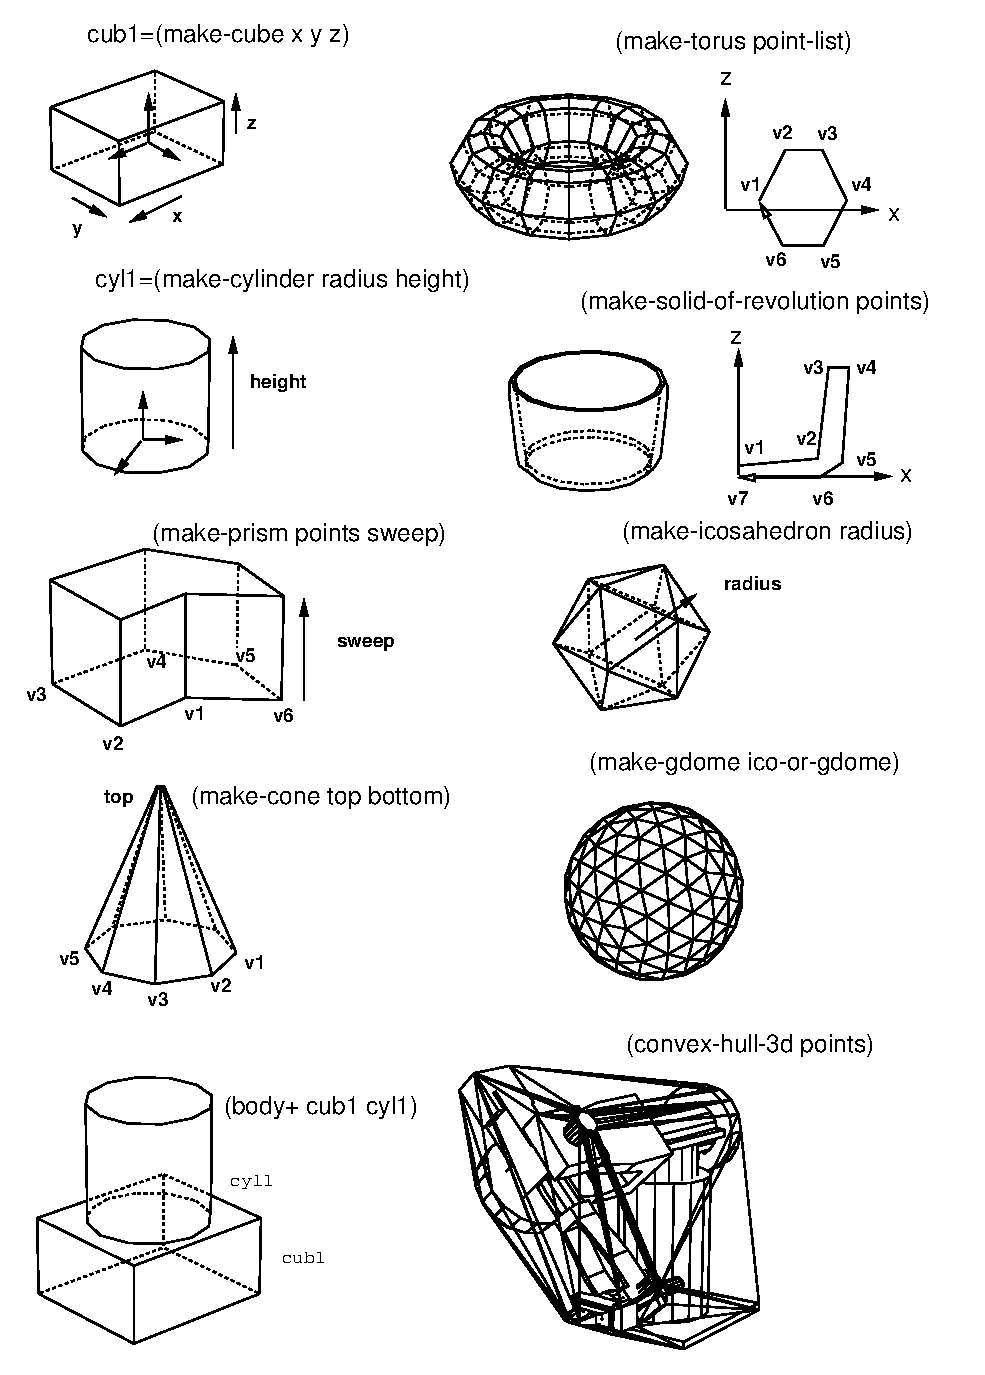
\includegraphics[width=10cm]{fig/fig1.ps}
%\epsfile{file=fig/fig1.ps,height=19cm}
%\mbox{
%\epsfsize=10cm
%\epsfbox[0 600 300 800]{fig/fig1.ps}
%\epsfbox{fig/fig1.ps}
%}
\end{center}
\caption{primitive bodies}
\end{figure}

\funcdesc{make-cube}{xsize ysize zsize \&key name color}{
makes a cuboid whose sizes in x, y and z directions are {\em xsize, ysize}
and {\em zsize}.
The coordinates origin of this cuboid locates at the center of the body.}

\funcdesc{make-prism}{bottom-points sweep-vector \&key name color}{
Makes a prism by lifting the shape defined by {\em bottom-points}
along {\em sweep-vector}.
If the {\em sweep-vector} is a number, not a float-vector,
it is taken as the height of the prism in the $z$ direction.
Bottom points must be ordered as they define the bottom face of the body.
For example,
 (make-prism '(\#f(1 1 0) \#f(1 -1 0) \#f(-1 -1 0) \#f(-1 1 0)) 2.0)
makes a cube of height 2.0.}

\funcdesc{make-cylinder}{radius height \&key (segments 12) name color}{
Makes a cylinder with specified {\em radius} and {\em height}.
The bottom face is defined on xy-plane and the coordinates origin is
located at the center of the bottom face.}

\funcdesc{make-cone}{top bottom \&key (segments 16) color name}{
makes a cone body whose summit is the {\em top}
and bottom face is the {\em bottom}.
{\em Top} is a 3D float-vector.
{\em Bottom} is either a list of vertices of the bottom face or a radius
(scalar). If it is the vertices list, it is order sensitive.
\verb~ (make-cone \#f(0 0 10) (list \#f(10 0 0) \#f(0 10 0) \#f(-10 0 0) 
\#f(0 -10 0)))~ makes a cone of a square bottom.}


\funcdesc{make-solid-of-revolution}{points \&key (segments 16) name color}{
{\em Points} are revolted along z-axis in the clock wise direction.
If two end points in the {\em points} list do not lie on z axis,
those points make circular faces. Thus,
{\tt (make-solid-of-revolution '(\#f(0 0 1) \#f(1 0 0)))}
makes a cone, and 
{\tt (make-solid-of-revolution '(\#f(1 0 1) \#f(1 0 0)))}
makes a cylinder.
The {\em points} are order-sensitive,
and are expected to be arranged from higher $z$ coordinate
to lower $z$.}

\funcdesc{make-torus}{points \&key (segments 16) name color}{
makes a torus, a donuts like object.
{\em Points} is a list of vertices on a cross-section.}

\funcdesc{make-icosahedron}{\&optional (radius 1.0)}{
Makes a regular body of twenty faces.
Each face is a regular triangle.}

\funcdesc{make-dodecahedron}{\&optional (radius 1.0)}{
Makes a regular body of twelve faces.
Each face is a regular pentagon.}

\funcdesc{make-gdome}{abody}{
By subdividing triangle faces of abody into four subfacets,
makes a geodesic dome as a new body. Abody should be an icosahedron
initially, and then the result of make-gdome can be given to make-gdome
recursively.
At each call, the number of faces of the Gdome increases
by the factor of four,
i.e. 20, 80, 320, 1280, 5120, etc.
}
\begin{quote}
\begin{verbatim}
(setq g0 (make-icosahedron 1.0))	; 20 facets
(setq g1 (make-gdome g0))		; 80 facets
(setq g2 (make-gdome g1))		; 320 facets
...
\end{verbatim}
\end{quote}

\funcdesc{grahamhull}{vertices \&optional (normal \#f(0 0 1))}{
Computes convex-hull for 2D points by Graham's algorithm. Slower than
quickhull.}

\funcdesc{quickhull}{vertices \&optional (normal \#f(0 0 1))}{
Computes convex-hull for 2D points by the binary search method.}

\funcdesc{convex-hull-3d}{vertices}{
Computes convex-hull for 3D points by gift-wrapping method.}
\funcdesc{make-body-from-vertices}{vertices-list}{
creates a body from lists of vertices each of which define
a loop of a face in the consistent order.}

\end{refdesc}

\subsection{\label{BodyComposition}Body Composition}

\begin{refdesc}

\fundesc{face+}{face1 face2}
\funcdesc{face*}{face1 face2}{
{\em face1} and {\em face2} are coplanar faces in 3D space.
{\bf face+} composes union of these faces and returns a face object.
If there is no intersection, original two faces are returned.
{\bf face*} returns intersection of these faces.
If there is no intersection, NIL is returned.}

\funcdesc{cut-body}{body cutting-plane}{
Cuts a body by the {\em cutting-plane}
and returns a list of faces made at the cross-section.}

\fundesc{body+}{body1 body2 \&rest more-bodies}
\fundesc{body-}{body1 body2}
\funcdesc{body*}{body1 body2}{
Computes join, difference or intersection of two or more bodies.
Each body is copied before each {\bf body+, body-} and {\bf body*} operation,
and original bodies are unchanged.
The new coordinates of the resulted body is located and oriented
at the same location and orientation as the world coordinates.
Even when two bodies are touching face by face,
these functions are expected to work correctly
if threshold parameters
{\tt *coplanar-threshold*, *contact-threshold*,} and {\tt *parallel-threshold*}
are properly set.
However, if a vertex of a body is in contact with an edge or a face
of the other body, any composition operation fails.}

\funcdesc{body/}{body plane}{
Cut the body by a plane which is an instance of class plane
(made by {\bf make-plane}).
A newly created body is returned.}

\funcdesc{body-interference}{\&rest bodies}{
Checks interference between each one-to-one combination in {\em bodies}.
Returns a list of two bodies  that are intersecting.
}

\end{refdesc}

\subsection{Coordinates-axes}
Class coordinates-axes defines 3D coordinates-axes drawable on a screen.
Each axis and an arrow at the tip of z-axis are defined by line objects.
Since the coordinates-axes class inherits cascaded-coords,
a coordinates-axes object can be attached
to another cascaded-coords originated object such as a body.
This object is used to see the coordinates-axes of a body or a
relative coordinates to another coordinates.

\begin{refdesc}
\classdesc{coordinates-axes}{cascaded-coords}
{(size model-points points lines)}{Defines drawable 3-D coordinates-axes.}
\end{refdesc}

\newpage

